\documentclass[lang=en]{sjtuarticle}
\title{Trusted LLM}  %: 
\author{Log Creative}
\sjtusetup{info/date={2024-06-11}}
\graphicspath{{figs/}}
\usepackage[style=ieee]{biblatex}
\addbibresource{ref.bib}
\usepackage[colorlinks]{hyperref}

\begin{document}
\maketitle

\tableofcontents*

\section{LLM}\label{sec:llm}

\begin{figure}[h]
    \centering
    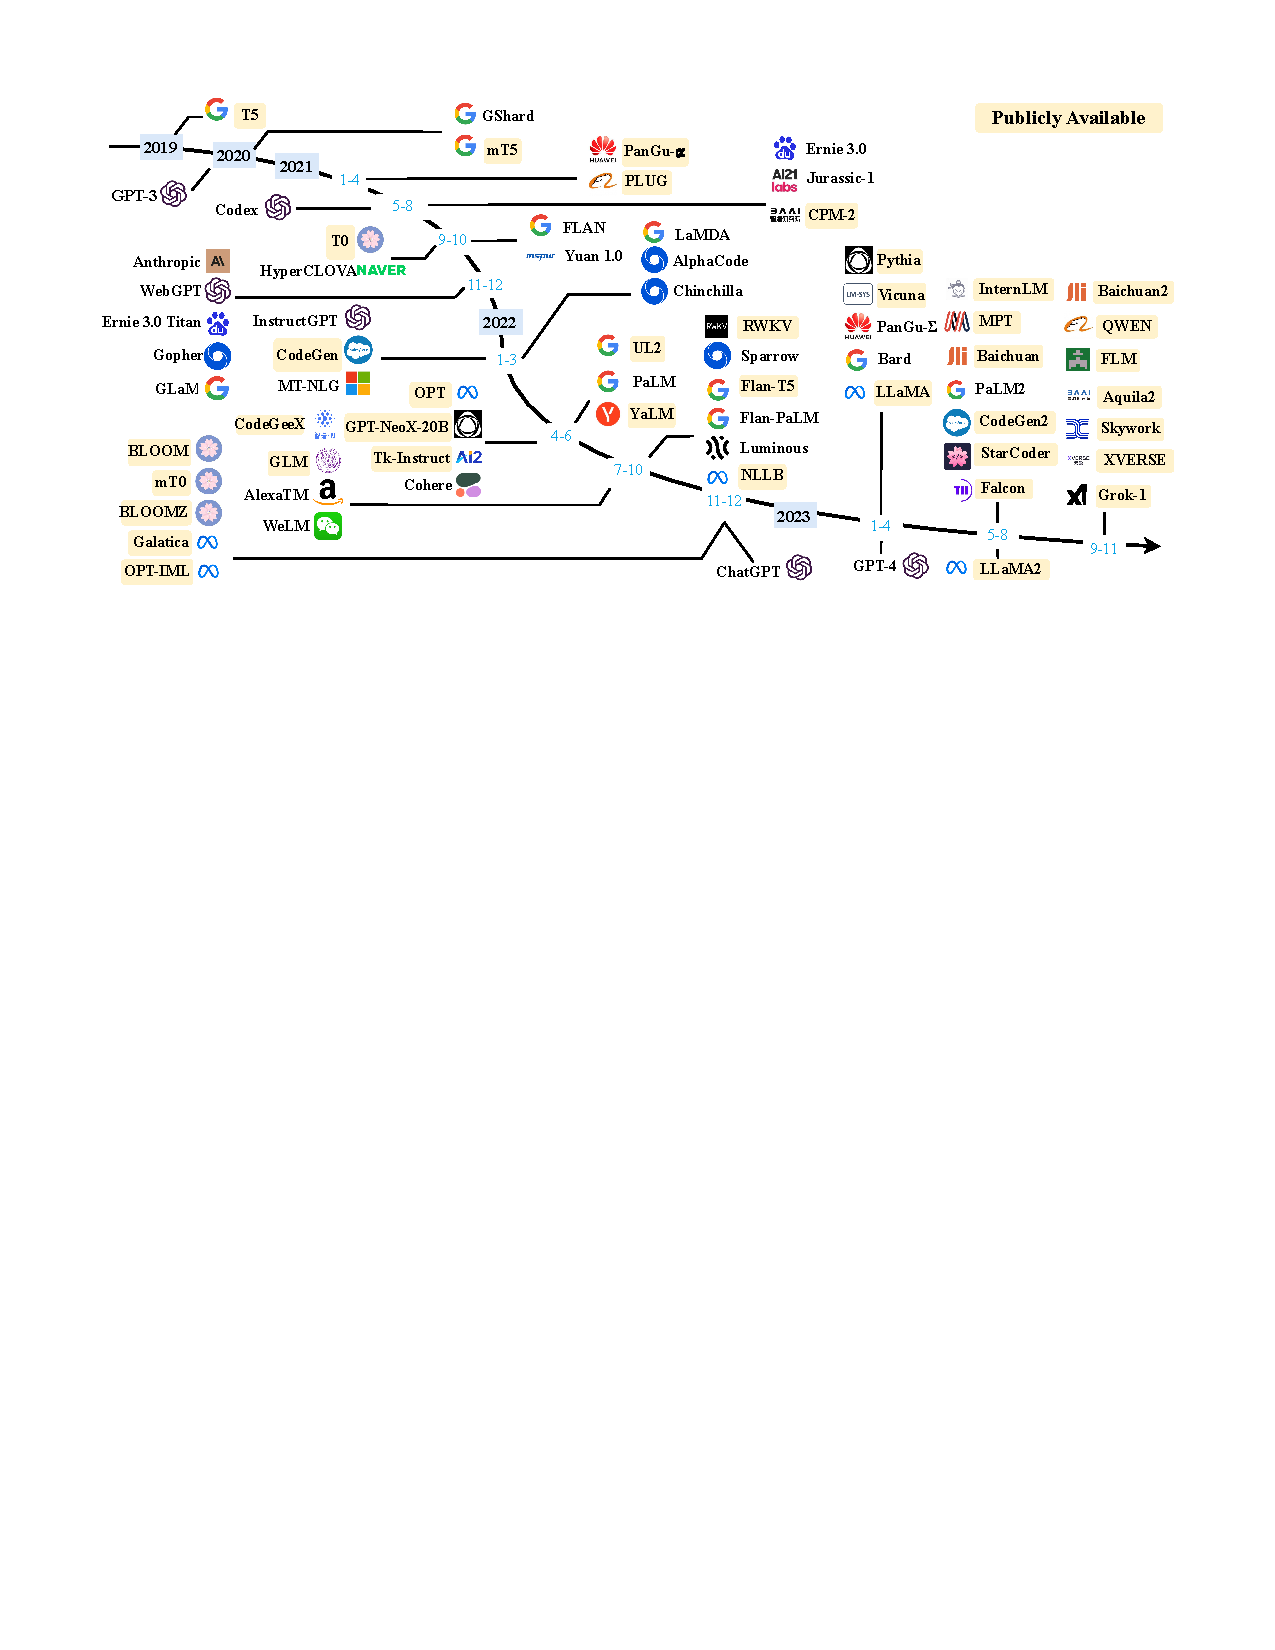
\includegraphics[width=\textwidth]{timeline.pdf}
    \caption{A timeline of existing large language models in recent years \cite{zhao2023survey}}
    \label{fig:timeline}
\end{figure}

\paragraph{NLP.}
NLP (Natural Language Processing) can be categorized into the subfields of AI (Artificial Intelligence) and linguistics. NLP mainly explores how to make machines understand,
process, reproduce, and generate natural languages \cite{chang2023natural}.

\paragraph{LLM.}
Large Language Models (LLMs) refer to Transformer \cite{transformer}
language models that contain hundreds of billions (or
more) of \textbf{parameters}, which are trained on massive text
\textbf{data}. The advent of LLMs (Large Language Models) marks a significant milestone in NLP and generative AI \cite{sun2024trustllm}, which have exhibited remarkable capabilities in tackling complex tasks, exemplified by
their ability to engage in human-like conversations as demonstrated by ChatGPT \cite{ouyang2022training}. Consequently, this has propelled
significant research endeavors shown in Figure \ref{fig:timeline} with blooming research accomplishments across both the open-source models and commercial models.

\paragraph{Applications of LLM.}
% and applications within domains such as finance and healthcare \cite{chen2023federated}. 
LLMs are revolutionizing a multitude of industries by their ability to process and generate human-like text. They are instrumental in enhancing \textbf{NLP tasks} such as translation, summarization, and question-answering. In \textbf{healthcare}, LLMs expedite literature retrieval and analysis, aiding in drug discovery and genomics. They also contribute to \textbf{robotics} by facilitating natural language understanding for robots, and in the field of \textbf{computer science}, they assist in code generation and debugging. Moreover, LLMs are being \textbf{fine-tuned or adapted} for specific applications, leading to more personalized and accurate responses, e.g., Apple Intelligence \cite{apple} could apply LLMs to Siri to help with everyday tasks based on the personal context and fine-tuned or adapted models shown in Figure \ref{fig:appleIntent}.  The rapid advancements in LLM research are continuously expanding their applications, making them a pivotal tool in the progression of AI \cite{naveed2023comprehensive}.

\begin{figure}[h]
    \centering
    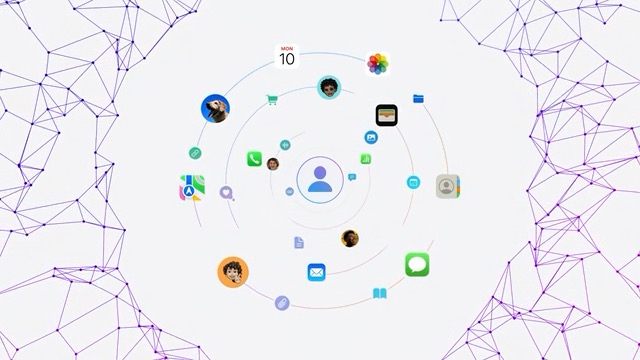
\includegraphics[width=0.7\textwidth]{appleContext.jpeg}
    \caption{Apple Intelligence could understand the intent of the user on everyday tasks based on LLM}
    \label{fig:appleIntent}
\end{figure}

\paragraph{Origin of LLMs' intelligence.}
The outstanding capabilities of LLMs can be attributed to multiple factors \cite{sun2024trustllm}, such as the usage of large-scale
raw texts from the Web as \textbf{training data} (e.g., PaLM \cite{anil2023palm} was trained on a large dataset containing more
than 700 billion tokens), the design of transformer architecture with \textbf{a large number of parameters} (e.g.,
GPT-4 \cite{achiam2023gpt} is estimated to have in the range of 1 trillion parameters), and advanced training schemes that
\textbf{accelerate the training process}, e.g., low-rank adaptation (LoRA) \cite{hu2021lora}, quantized LoRA \cite{dettmers2024qlora}, and pathway
systems \cite{barham2022pathways}. Moreover, their outstanding instruction following capabilities can be primarily attributed to the
implementation of \textbf{alignment with human preference}. Prevailing alignment methods use reinforcement
learning from human feedback (RLHF) \cite{ouyang2022training}, which shapes the behavior of LLMs to more closely align with
human preferences, thereby enhancing their utility and ensuring adherence to ethical considerations.

\paragraph{Trustworthy challenges of LLMs.}

However, the rise of LLMs also introduces concerns about their trustworthiness. Unlike traditional language
models, LLMs possess unique characteristics that can potentially lead to trustworthiness issues. There are mainly 6 dimensions concerning the trustworthiness of LLMs \cite{sun2024trustllm}:

\begin{itemize}
    \item \textbf{Truthfulness.} Truthfulness in AI systems refers to the accurate representation of information, facts, and
    results. LLMs tend to have hallucinations in a dialog where misinformation or outdated information could be provided, which is primarily due to the noise in the training data and the lack of generalization capability in the Transformer architecture.
    \item \textbf{Safety.} Safety in LLMs is crucial for avoiding unsafe or illegal outputs and ensuring engagement in healthy
    conversations. LLMs could be jailbroken by attacks to output knowledge that is illegal or toxic, which is due to the sophisticated prompt engineering and the lack of safety protocols under the hood.
    \item \textbf{Fairness.} Fairness is the ethical principle of ensuring that LLMs are designed, trained, and deployed in ways
    that do not lead to biased or discriminatory outcomes and that they treat all users and groups equitably. The biased information could be outputted due to data biases and private
    information in large training datasets.
    \item \textbf{Robustness.} Robustness is defined as a system's ability to maintain its performance level under various
    circumstances. This is mainly related to the deployment architecture of LLMs to make the throughput available most of the time to meet high user expectations.
    \item \textbf{Privacy.} Privacy encompasses the norms and practices aimed at protecting human autonomy, identity, and
    dignity. (1) For individuals, in the absence of stringent safeguards, sensitive personal information within the
    training dataset becomes susceptible to misuse, potentially
    leading to privacy breaches. This issue is especially acute in the healthcare sector, where maintaining the
    confidentiality of patient data is of utmost importance \cite{chen2023federated}. (2) For companies, private domains have accumulated substantial volumes of data through
    advancements in AI algorithms. Nevertheless, privacy concerns and commercial competition tend to isolate such data
    sources, hindering direct collaboration and knowledge sharing. What's more, real-world data privacy regulations
    frequently impose restrictions on direct data sharing among isolated entities, thereby exacerbating concerns relating to
    data scarcity and privacy protection.
    \item \textbf{Machine Ethics.} Machine ethics ensure the moral behaviors of man-made machines utilizing AI, commonly
    referred to as AI agents. This is mainly related to the ethical property of the training data.
\end{itemize}

As a result, \textbf{data privacy} and \textbf{correct execution} (output the desired information) are key challenges for trusted LLMs. LLM is of a great scale, as a result, the \textbf{efficiency} often matters.

\section{Trusted LLMs}

The next-generation internet, with its focus on trusted identity (entity authentication, identity management and system), trusted data (message authentication, blockchain and oracle), and trusted computation (multiparty computation, verifiable computing, smart contract and TEE-based computing), is expected to significantly influence the field of LLM to tackle the challenges mentioned in Section \ref{sec:llm}. This paper mainly focuses on \textbf{trusted computation} for LLM to preserve the privacy of data and prove the correctness of execution.

\paragraph{Data privacy.}
Addressing the challenge of utilizing private domain data for modeling purposes, while simultaneously upholding
data privacy, is an issue of great significance. Existing solutions tackle this problem by employing privacy-preserving
computation techniques. Three primary approaches to privacy-preserving computation are currently prevalent \cite{chen2023federated}: (1)
cryptography-based methods that primarily focus on secure multi-party computation (SMPC); (2) confidential
computing, which utilizes trusted hardware such as trusted execution environments (TEE); (3) federated learning
(FL), a technique that integrates privacy-preserving measures into collaborative modeling. Section \ref{sec:mpc} and Section \ref{sec:tee} will introduce the current state-of-the-art. Those methods are expected to be used widely to construct LLMs with more trustworthiness.

\paragraph{Correct execution.} As laws and regulations around LLMs evolve
and tighten, developing practical tools to verify the legitimacy of
these models has become crucial. Section \ref{sec:zkllm} will introduce the proving method based on zero-knowledge proof.

\subsection{Sigma: LLM with efficient 2PC}\label{sec:mpc}

2PC (2-party computation), which is a specific scenario of MPC (multi-party computation), could be described as follows. There
are two parties $P_0$ and $P_1$ with inputs $x_0$ and $x_1$ and they wish to
compute a public function $y=f(x_0,x_1)$ without revealing anything
more than the function output $y$ to each other. In a preprocessing
phase that is independent of the inputs to the function $x_0$ and $x_1$,
correlated randomness is generated and made available to $P_0$ and
$P_1$.

While SMPC (secure multi-party computation) ensures robust security, it may not
adequately address efficiency requirements. Sigma \cite{cryptoeprint:2023/1269} is a system that advances the
state-of-the-art for secure inference of transformer-based models
along multiple dimensions. Like CrypTen \cite{NEURIPS2021_27545182}, Sigma works in 2PC with
preprocessing model and uses GPU acceleration, but is an order
of magnitude \textbf{more efficient} in latency and communication while
providing standard 2PC security guarantees. Sigma maintains the model accuracy under secure inference through precise approximations of complex non-linearities and scales efficiently to GPT
models with billions of parameters.

Function secret sharing (FSS) \cite{boyle2016function} is a
recent paradigm for obtaining efficient 2PC protocols with a preprocessing phase. Sigma is the first end-to-end system
for secure transformer inference based on FSS. By constructing
new FSS-based protocols for complex machine learning functionalities, such as Softmax, GeLU and SiLU, and also accelerating their
computation on GPUs, Sigma improves the latency of secure inference of transformers by $11-19\times$ over the state-of-the-art that
uses preprocessing and GPUs. Sigma is the first secure inference
of GPT models, which shows the potential of MPC in use on LLMs.

\subsection{Federated LLM with TEE}\label{sec:tee}

LLMs integrated with Trusted Execution Environments (TEEs) represent a significant advancement in secure computing. TEEs provide a secure area of the main processor that guarantees the confidentiality and integrity of the code and data loaded inside it. LLMs with TEE could have the following benefits:

\begin{itemize}
    \item \textbf{Data Privacy.} TEEs can ensure that sensitive data used by LLMs, such as personal information or proprietary business data, is processed securely, preventing unauthorized access and leaks.
    \item \textbf{Model Protection.} LLMs often contain proprietary algorithms and structures. TEEs can protect these models from being reverse-engineered or tampered with, preserving intellectual property.
    \item \textbf{Secure Inference.} When LLMs perform inference tasks, TEEs can ensure that the computation is performed in a secure environment, which is crucial for applications in sensitive domains like healthcare or finance.
    \item \textbf{Auditability and Compliance.} With TEEs, it's possible to provide verifiable logs of LLM operations, which can be crucial for regulatory compliance and audit trails.
\end{itemize}

Meanwhile, the distributed (federated) LLM is an important method for
co-training the domain-specific LLM using siloed data. However, maliciously stealing model parameters and data from
the server or client side has become an urgent problem to
be solved. TEEs can facilitate secure federated learning, where multiple parties collaboratively train an LLM without exposing their individual datasets. This is particularly useful for privacy-preserving distributed learning scenarios. \cite{huang2024fast} proposes a secure distributed
LLM based on model slicing with secure communication executed in the TEE and general environments through
lightweight encryption.

\begin{figure}[h]
    \centering
    \begin{subfigure}{.45\textwidth}
        \centering
        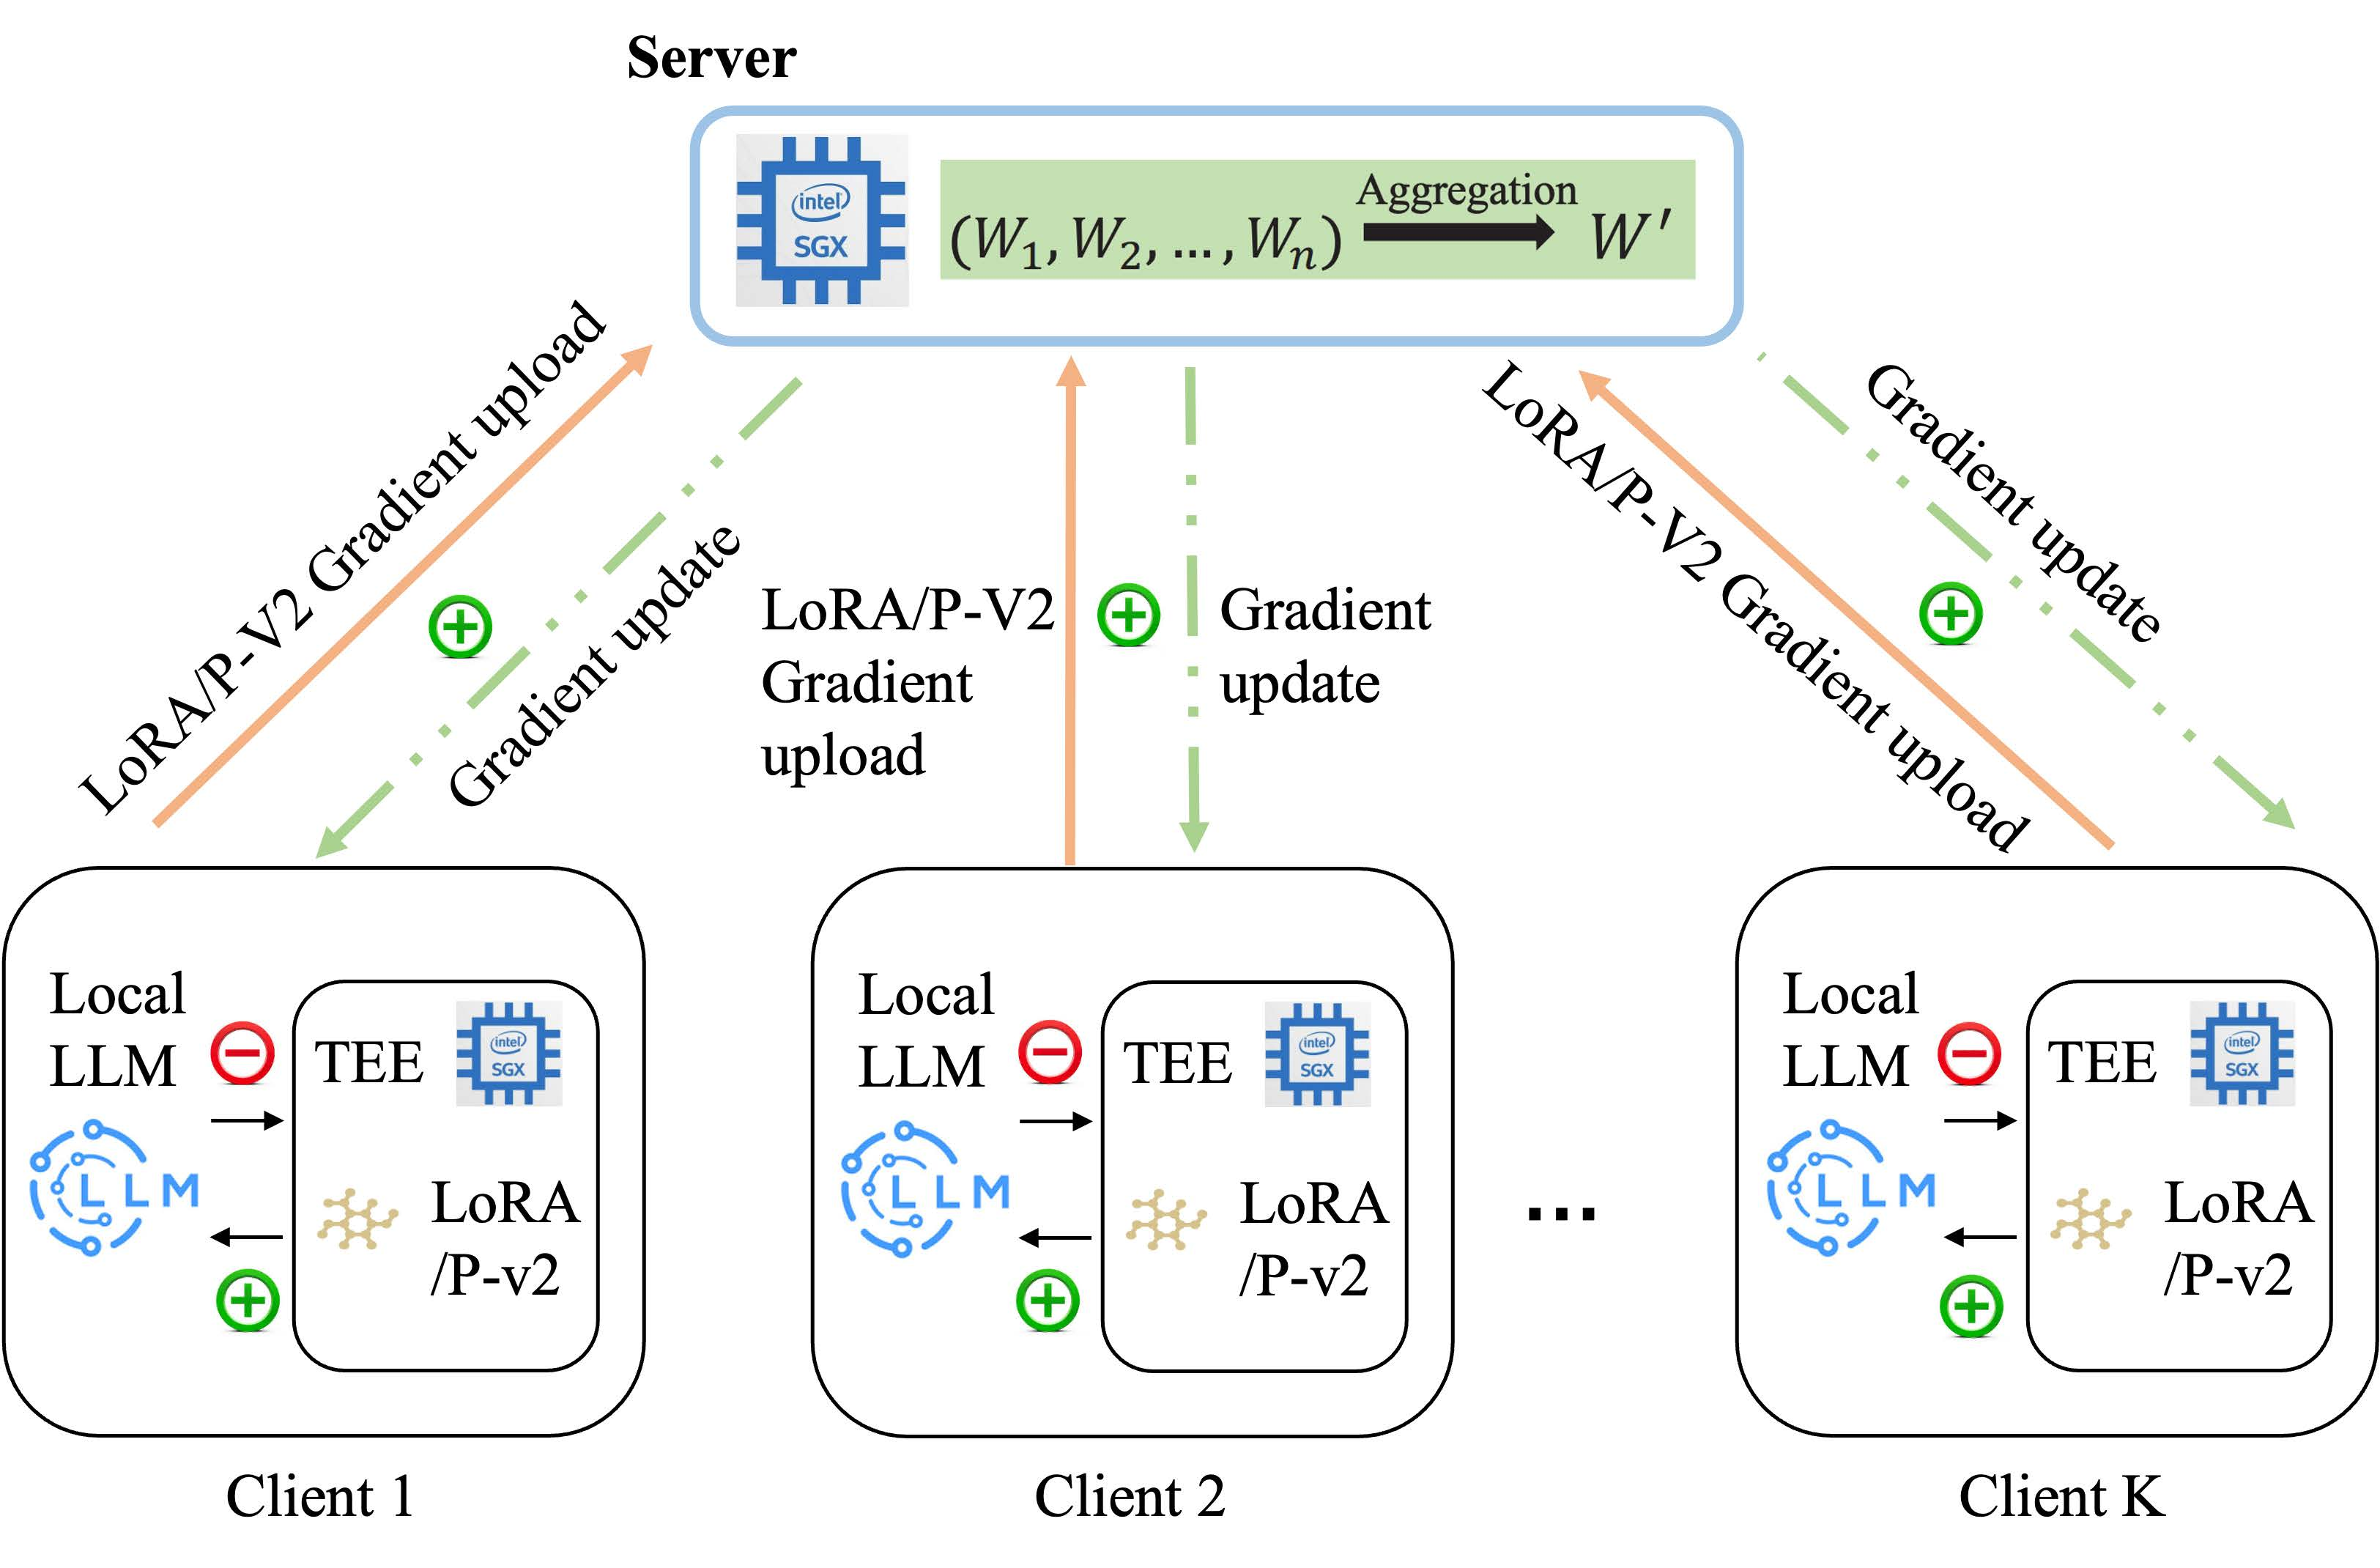
\includegraphics{llmtee.jpg}
        \caption{Method 1}
        \label{fig:llmtee1}
    \end{subfigure}\hfill
    \begin{subfigure}{.45\textwidth}
        \centering
        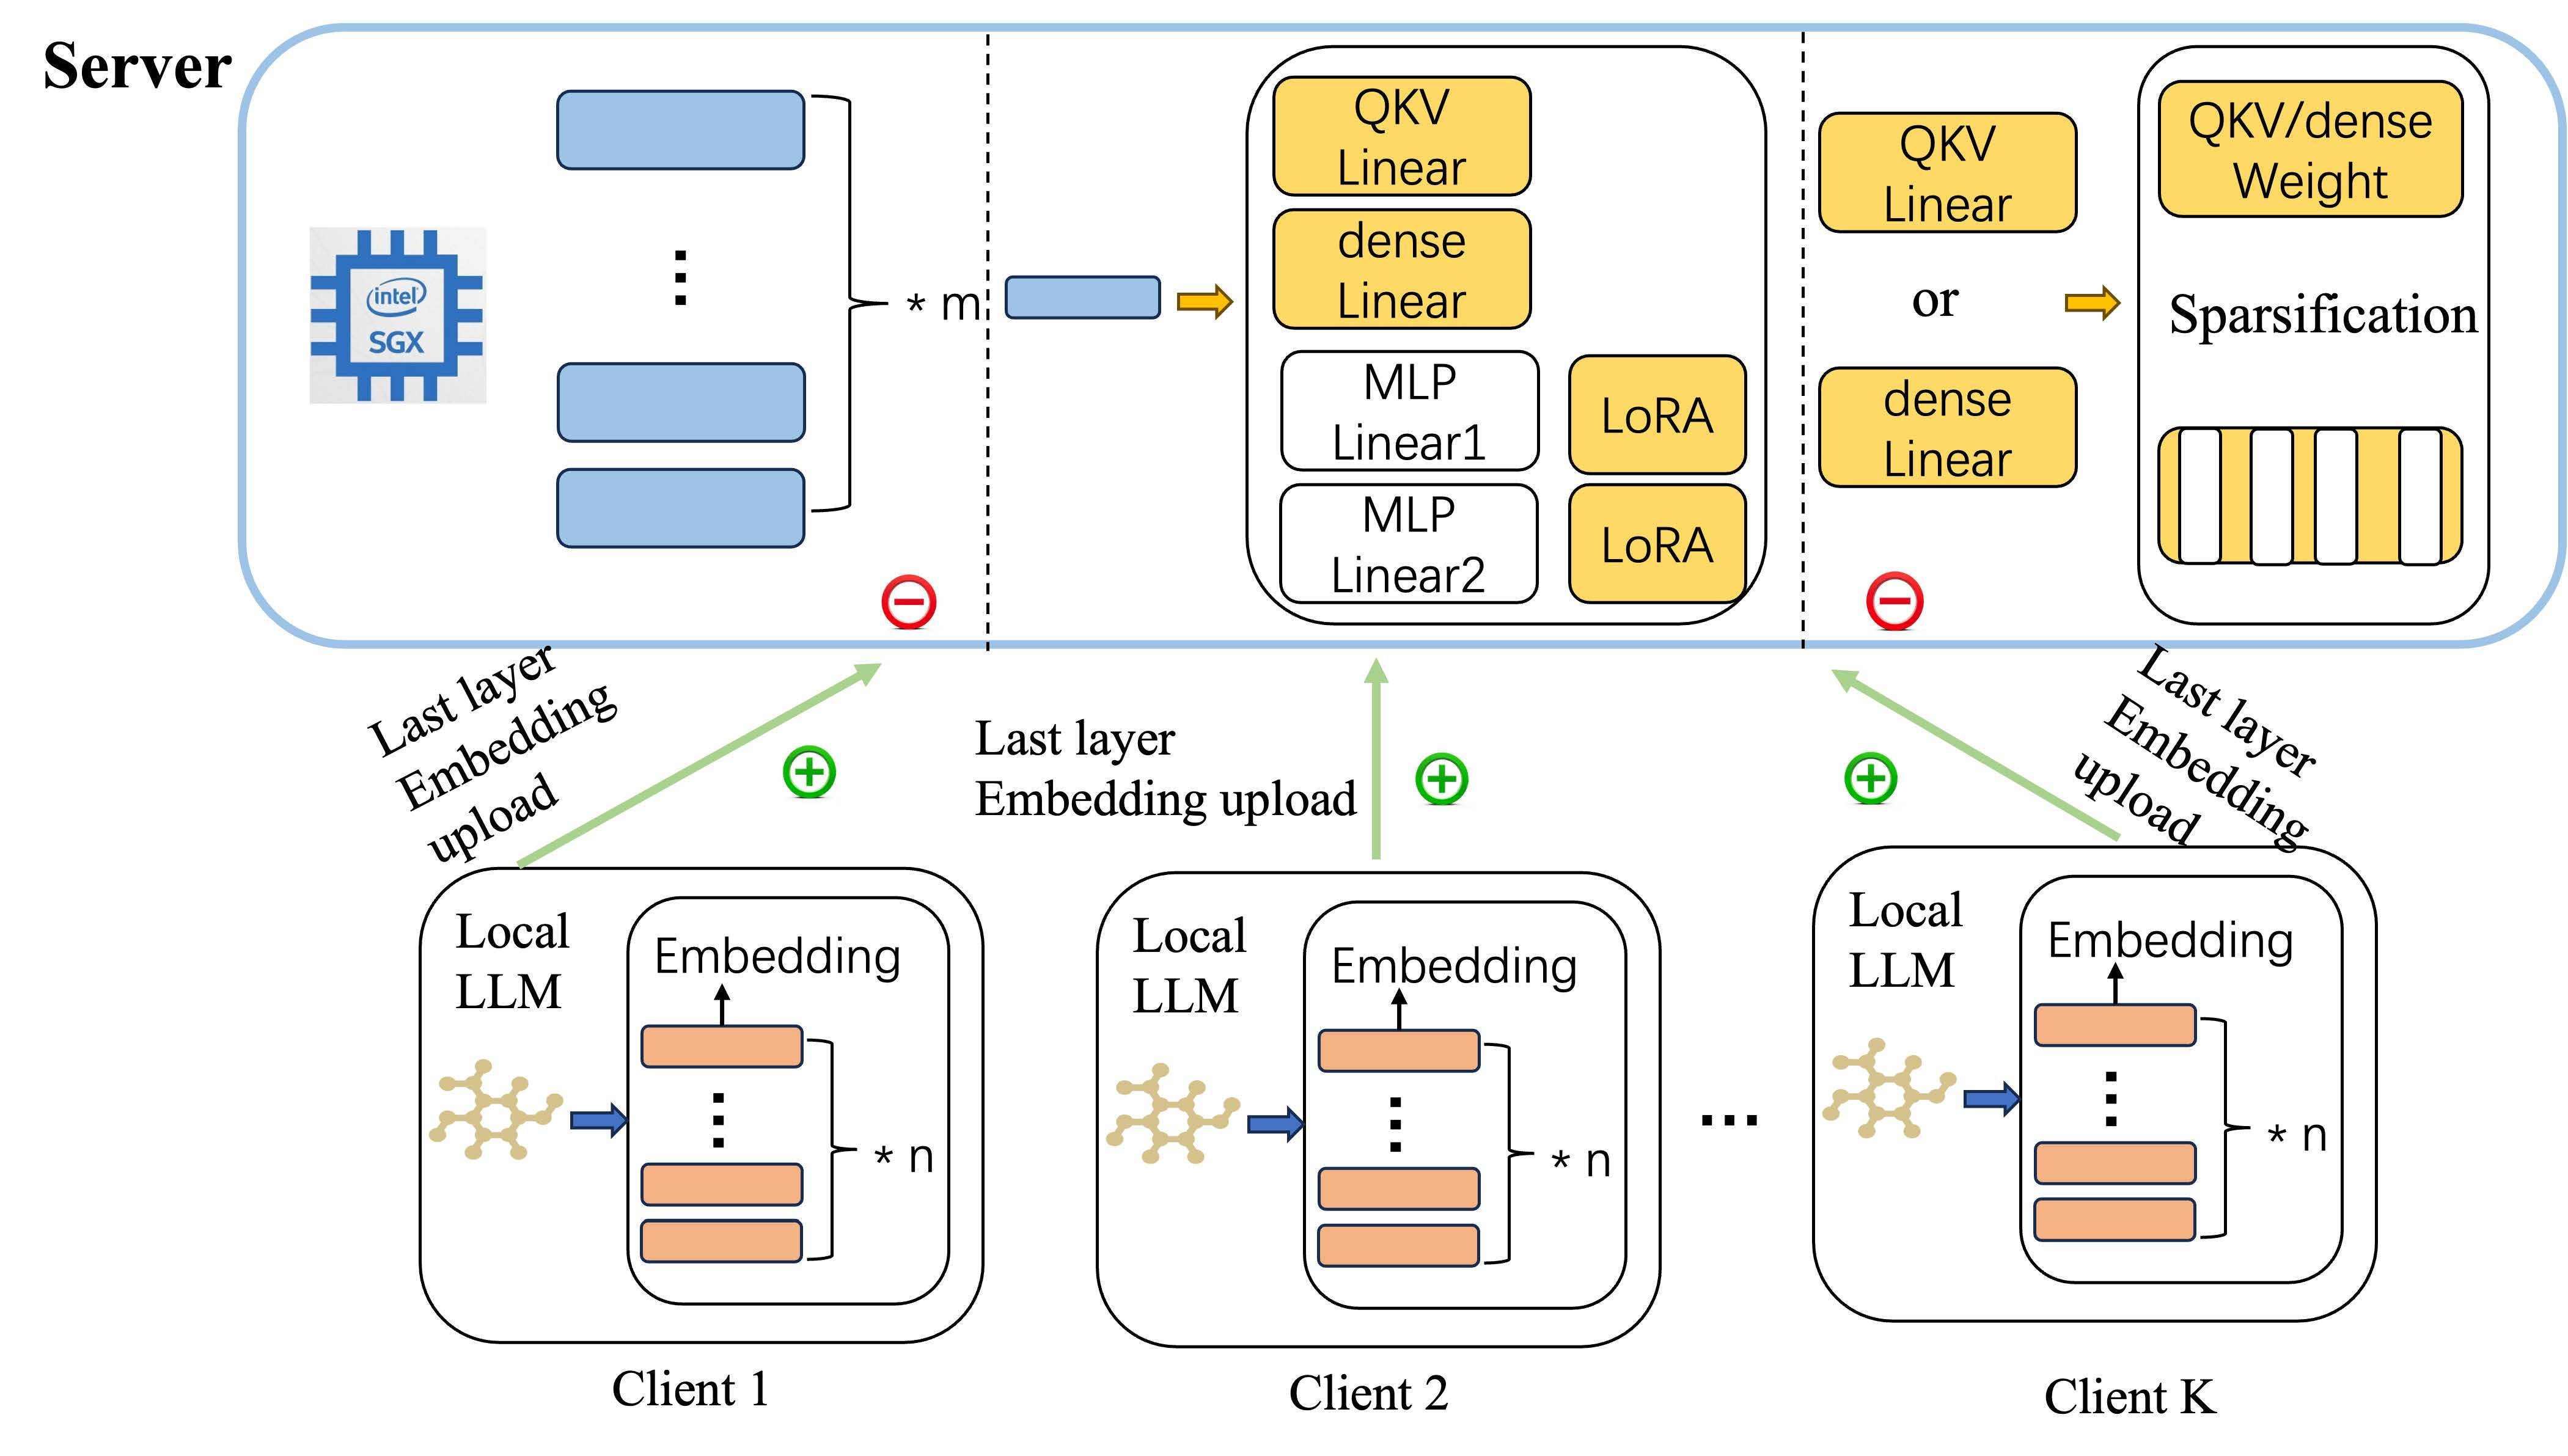
\includegraphics[width=\textwidth]{llmtee2.jpg}
        \caption{Method 2}
        \label{fig:llmtee2}
    \end{subfigure}
    \caption{Block diagram of the distributed LLM, where the green plus sign indicates encryption and the red minus sign indicates decryption.}
    \label{fig:llmtee}
\end{figure}

Shown in Figure \ref{fig:llmtee}, \cite{huang2024fast} proposes two methods: (a) Method 1 slices the LLM, deploys the sensitive part of the
structure in the TEE, and protects the transmission between
the TEE and GPU through OTP (One Time Pad) \cite{tramer2018slalom} to achieve the protection effect
of the model parameters and data. (b) In Method 2, after each
client collects the embedding of all the data, it is uploaded
to the server's TEE using OTP encryption. The server's
TEE receives the data and does the decryption for further finetuning the
model.

Both methods have pros and cons. Method 1 is for small memory (consumer-grade) TEE-shielded
LLM Partition; while Method 2 is for large memory TEE-shielded LLM Partition. Method 1 solves the security problem, but its client generates
a higher number of transmissions between the GPU and TEE
during training. Secondly, during the process of encryption
and decryption, there is a loss of numerical accuracy due to
truncation errors, resulting in a slight degradation of accuracy. It is ideal to use Method 2 when the device is of industry grade.

Furthermore, Apple Intelligence \cite{apple}, shown in Figure \ref{fig:apple}, also makes use of TEEs (marked as Secure Enclave in the figure) to provide the Private Cloud Compute (PCC) feature of LLMs and other large-scale models on both the on-device side and the Apple silicon server side. It is very promising for TEE to be widely used in federated LLM inferencing!

\begin{figure}[h]
    \centering
    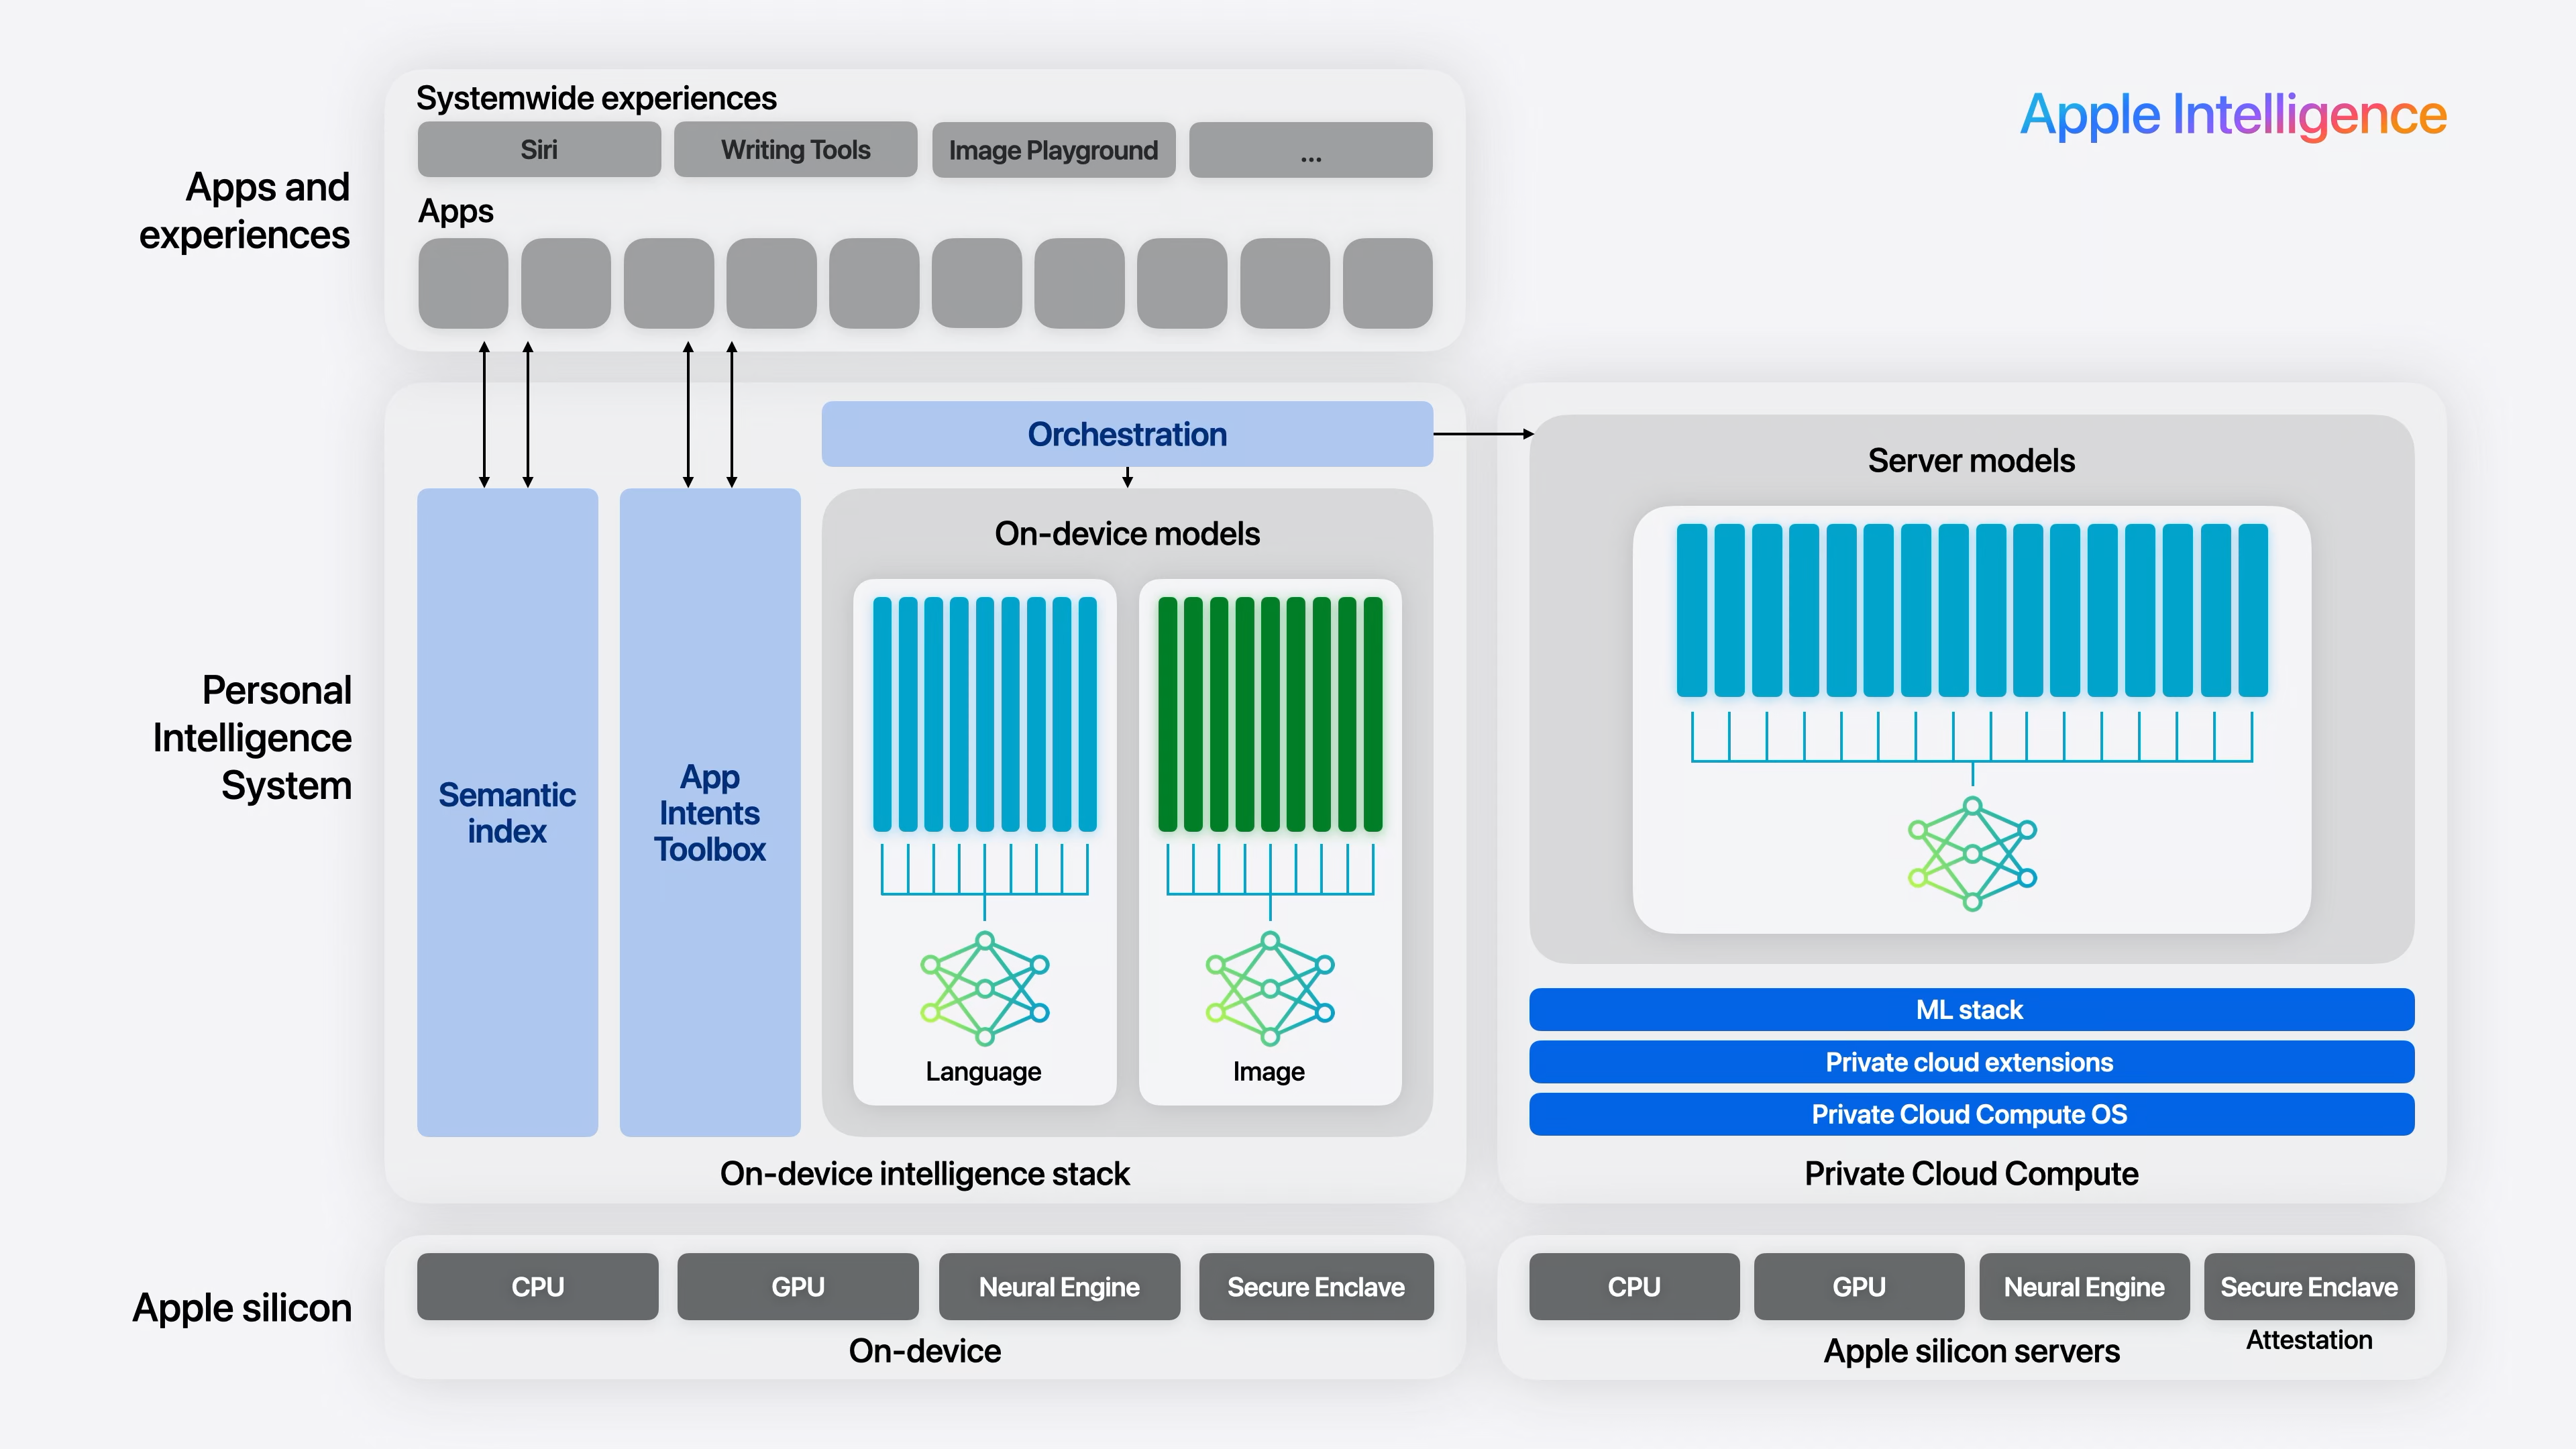
\includegraphics[width=\textwidth]{AppleIntelligence.png}
    \caption{The architecture of Apple Intelligence \cite{apple}}
    \label{fig:apple}
\end{figure}

\subsection{zkLLM}\label{sec:zkllm}

Because ML (Machine Learning) is deployed
behind these closed systems, there are increasing calls for
transparency, such as releasing model weights. However,
these service providers have legitimate reasons not to release
this information, including for privacy and trade secrets.
To bridge this gap, recent work has proposed using zero-knowledge
proofs (ZKPs)
for certifying computation with private models \cite{chen2024zkml}.

However, adapting existing ZKP techniques to modern LLMs,
characterized by their immense scale, presents significant challenges.
These models require substantial computational resources,
which general-purpose ZKP frameworks,
often unaware of LLM structure and limited in parallel computation
support, struggle to provide.

For LLMs specifically, zkLLM \cite{sun2024zkllm} can address challenges related to the legitimacy of model outputs, offering solutions for non-arithmetic operations in deep learning and enabling zero-knowledge proofs for the attention mechanism (called \textsf{zkAttn}, which leveraging
the foundation of \textsf{tlookup}). This can lead to the generation of correctness proofs for LLM inference processes, maintaining the privacy of model parameters while ensuring the integrity of the computations. Since zkLLM is implemented in CUDA, zkLLM emerges as a significant stride towards achieving efficient
zero-knowledge verifiable computations over LLMs.

\paragraph{\textsf{zkAttn}.} It is to achieve zero-knowledge verifiability with limited overhead
for the attention mechanism, shown in Figure \ref{fig:zkattn}.

\paragraph{\textsf{tlookup}.} It is the foundation of \textsf{zkAttn}. It is to address
general non-arithmetic operations in deep learning. The
\textsf{tlookup} design preserves the widely-used tensor-based structure,
guaranteeing seamless compatibility with the established computational
frameworks in deep learning. The protocol is shown in Figure \ref{fig:tlookup}.

\begin{figure}[h]
    \centering
    \begin{minipage}{.4\textwidth}
        \centering
        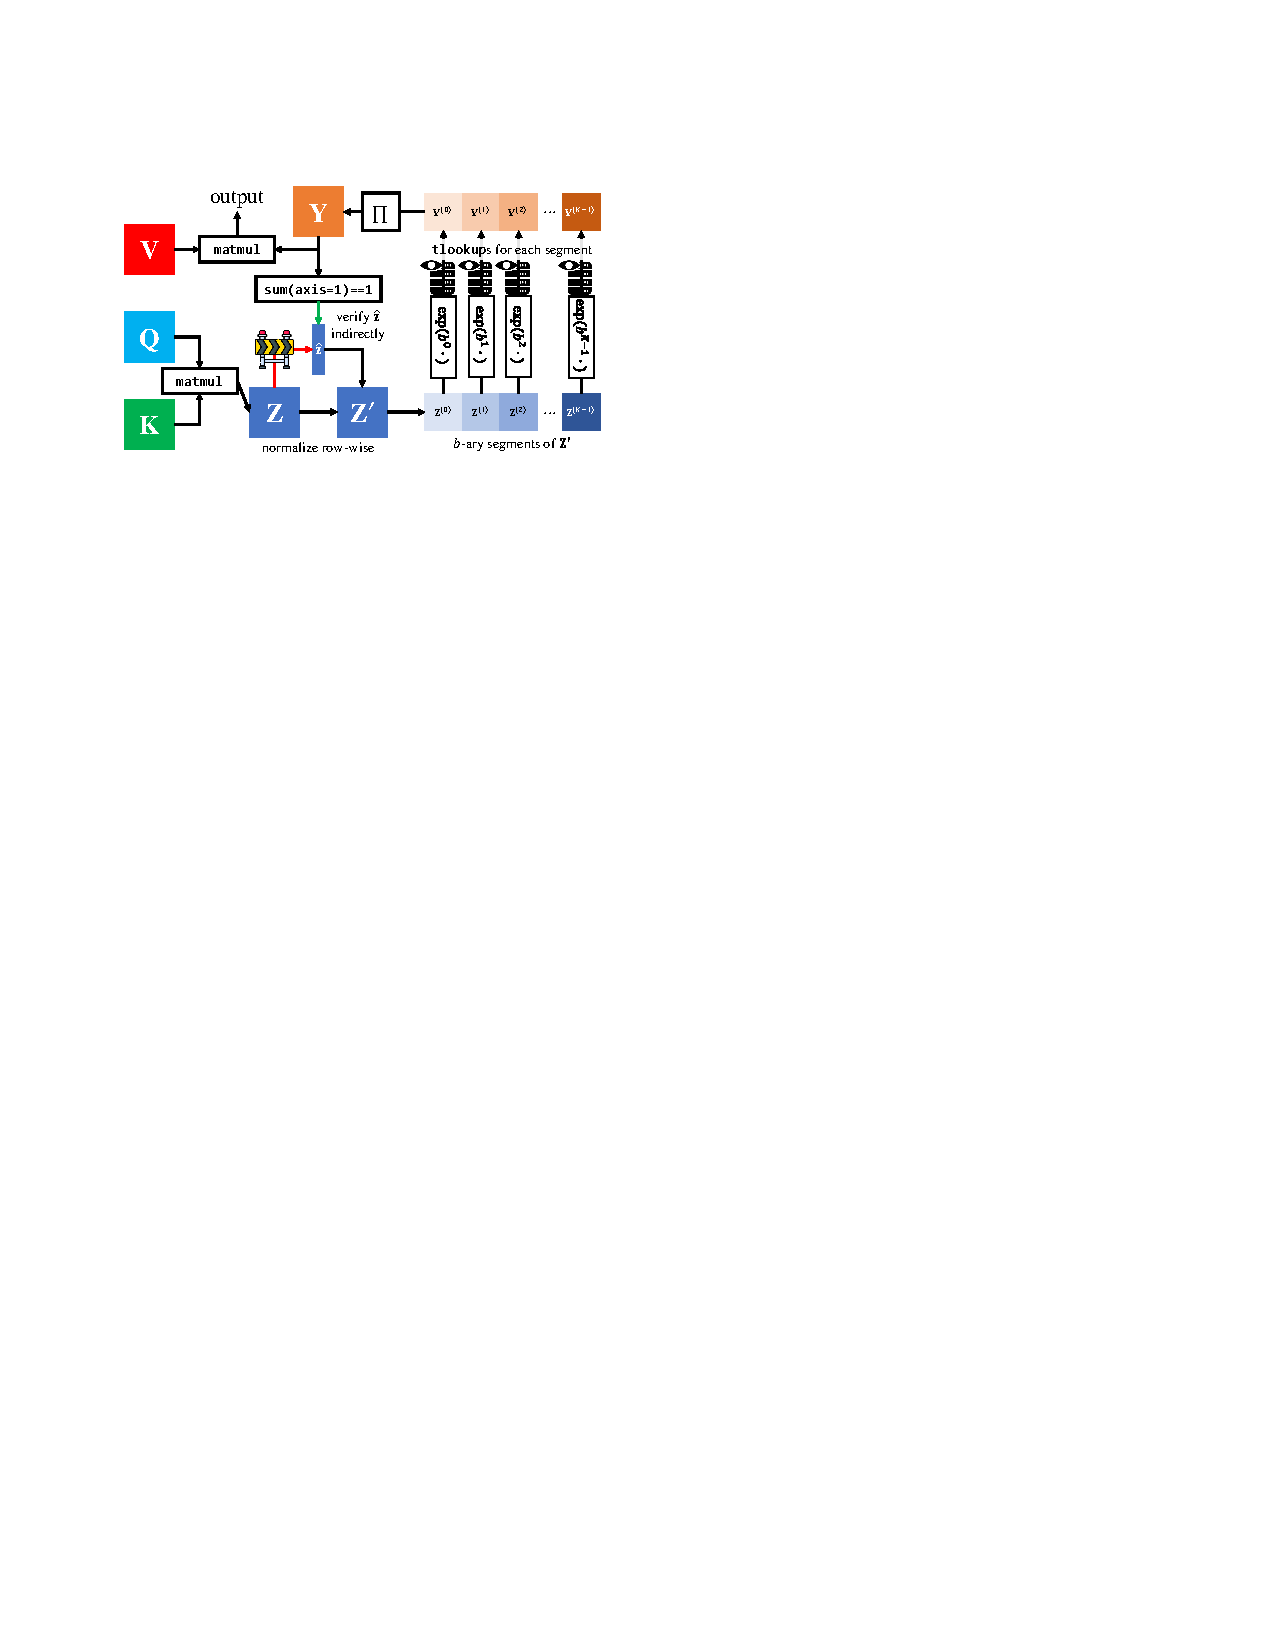
\includegraphics[width=\textwidth]{zkattn.pdf}
        \caption{Overview of \textsf{zkAttn}}
        \label{fig:zkattn}
    \end{minipage}\hfill
    \begin{minipage}{.55\textwidth}
        \centering
        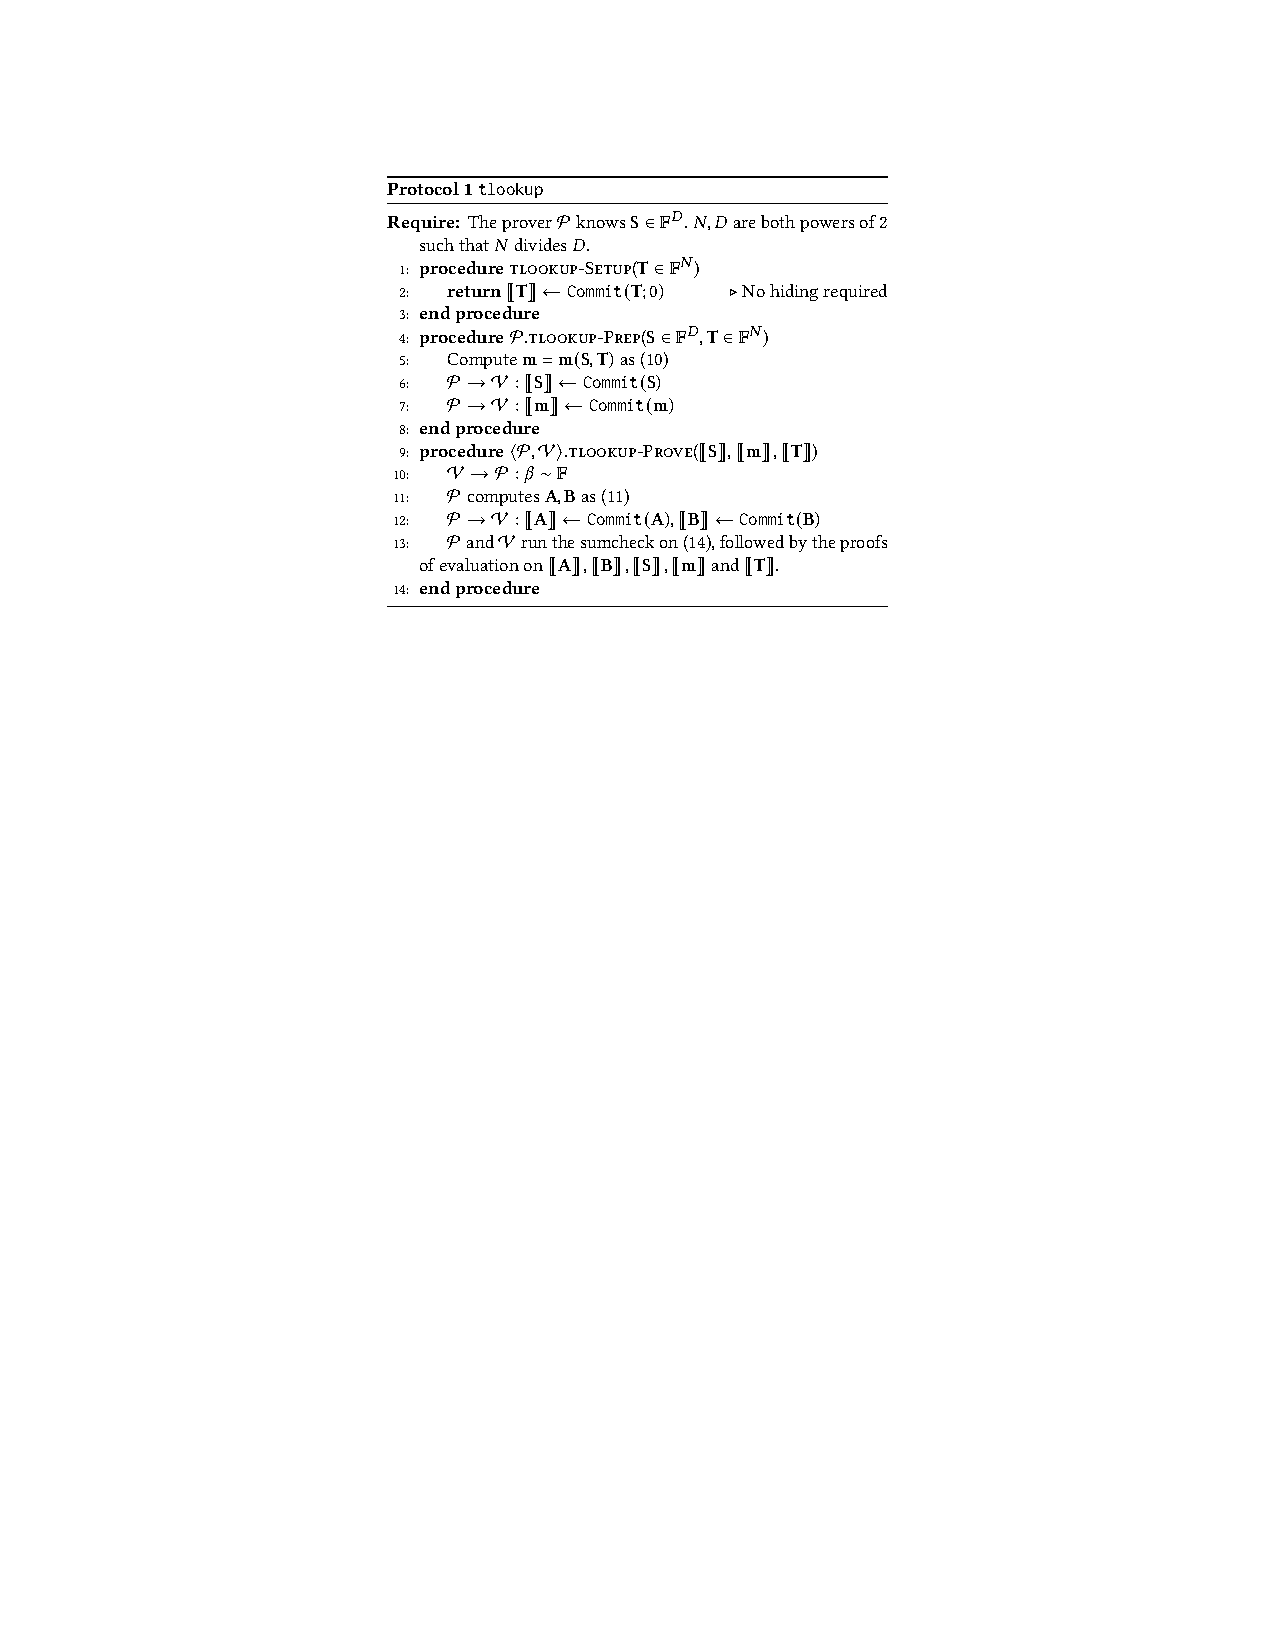
\includegraphics{tlookup.pdf}
        \caption{\textsf{tlookup}}
        \label{fig:tlookup}
    \end{minipage}
\end{figure}

In summary, ZKP could be used in LLM to fortify the legitimacy of LLMs
in light of their transformative impact on various domains with this promising design of zkLLM.

\section{Conclusion}

This paper first introduces LLM in the field of NLP, which has been applied in many areas of our daily lives. Considering the unique characteristics of LLM with a large number of parameters and training data, and unique training or finetuning methods, LLM faces data privacy and correct execution challenges in the aspect of trustworthiness, as well as the efficiency to provide such trusted LLM features.

The next generation of the Internet could come to help. This paper mainly focuses on trusted computation methods for trusted LLM: (a) Sigma \cite{cryptoeprint:2023/1269} provides an efficient method based on FSS to perform 2PC for LLM; (b) \cite{huang2024fast} provides federated methods to secure the computation of LLM inside TEEs. Apple Intelligence \cite{apple} also shows the potential to provide secure LLM feedback based on federated learning with TEEs. (c) zkLLM \cite{sun2024zkllm} provides an architecture to provide zero-knowledge proof of private LLM inferencing, which could fortify the legitimacy while keeping the model parameters secret.

It is promising for more LLMs to make use of the components of trusted computing to provide services with better privacy and provable safety, which is a great cross-innovation for the field of security with NLP!

\printbibliography

\end{document}